

\section{Introduction}

Recently, transformer-based language models 
have stretched notions of what is possible with the simple self-supervised objective of language modeling, becoming
a fixture in state of the art language technologies
\citep{vaswani2017attention, devlin-etal-2019-bert, brown2020language}.
However, the black box nature of these models combined with the complexity of natural language makes it
challenging to measure how accurately they
represent the world state underlying the text.

In order to better measure the extent to which these models can capture the world state underlying the symbolic data they consume, we propose training and studying
transformer language models for the game of chess.
Chess provides a simple, constrained, and deterministic domain where the exact world state is known.
Chess games can also be transcribed exactly and unambiguously using chess notations (Section~\ref{sec:chess}).
Most importantly, the form of chess notations allows us to probe our language models for aspects of the board state using simple prompts (Section~\ref{sec:probing}) and without changing the language modeling objective or introducing any new classifiers.\footnote{Code and data available at - \url{https://github.com/shtoshni/learning-chess-blindfolded}}



Due to the simplicity and precision of chess, we can evaluate language model predictions at a more fine-grained level than merely comparing them to the ground truth.
For example, even if the next move prediction doesn't match the ground truth move, we can still evaluate whether the move is legal given the board state, and if it is illegal, the error can be automatically analyzed (Appendix~\ref{sec:error_analysis}).
Moreover, since world state transitions are deterministic and known, we can  evaluate models using counterfactual queries as well.
Our proposed evaluation sets and metrics are described in Section~\ref{sec:cloze}.



While chess represents a controlled domain,
it is by no means trivial for a language model.
To illustrate the challenges of language modeling for chess,
consider the left board shown in Figure~\ref{fig:move_notation}, where white is next to move.
In order to generate a valid next move, the language model needs to (a) infer that it is white's turn, (b) represent the locations of all pieces, both white and black, (c) select one of the white pieces which can be legally moved, and finally (d) make a legal move with the selected piece.
Thus, a language model has to learn to track the board state, learn to generate moves according to the rules of chess, and on top of that learn chess strategies to predict the actual move. %


We find that when given enough training data, transformers can learn to both track piece locations and predict legal moves with high accuracy.
However, when trained on small training sets, predictive ability suffers. 
In this more challenging setting, introducing parts of the board state as tokens in the training sequences (Section~\ref{sec:rap_board})  improves piece tracking significantly (Appendix~\ref{sec:error_analysis}). 


\begin{figure*}
\begin{subfigure}{0.3\textwidth}
   \includegraphics[width=\linewidth]{figures/algebraic_notation.pdf}
   \caption{Square naming} \label{fig:algebraic_notation}
\end{subfigure}
\hspace*{\fill}
\begin{subfigure}{0.63\textwidth}
\begin{subfigure}{0.43\textwidth}
   \vspace{.2in}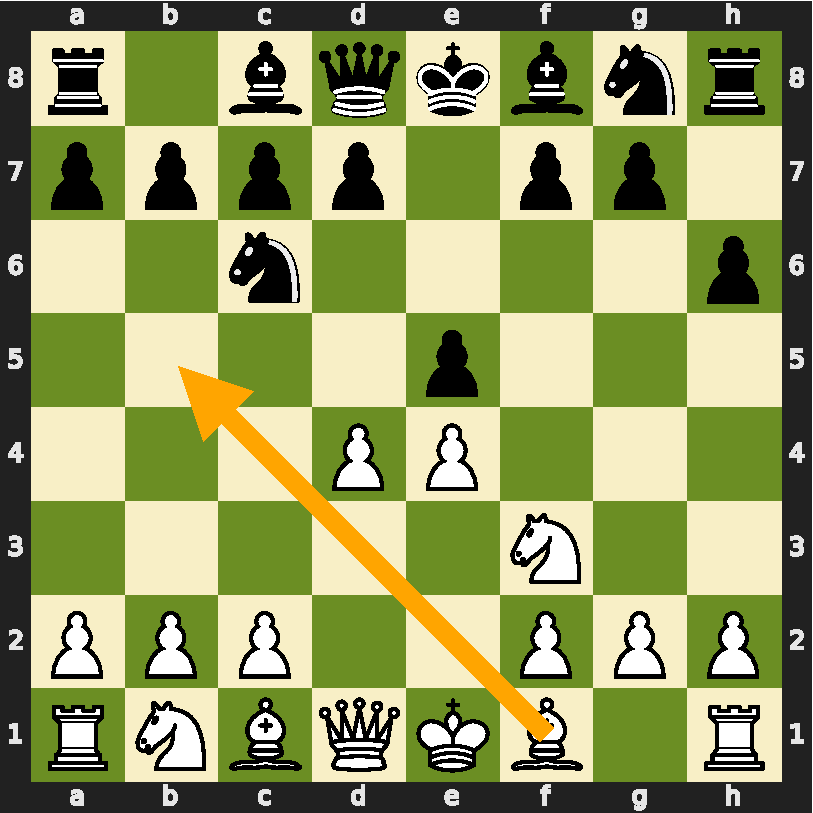
\includegraphics[width=\linewidth]{figures/board_prev.pdf}
\end{subfigure}
\hspace*{\fill}
\begin{subfigure}{0.43\textwidth}
   \vspace{.2in}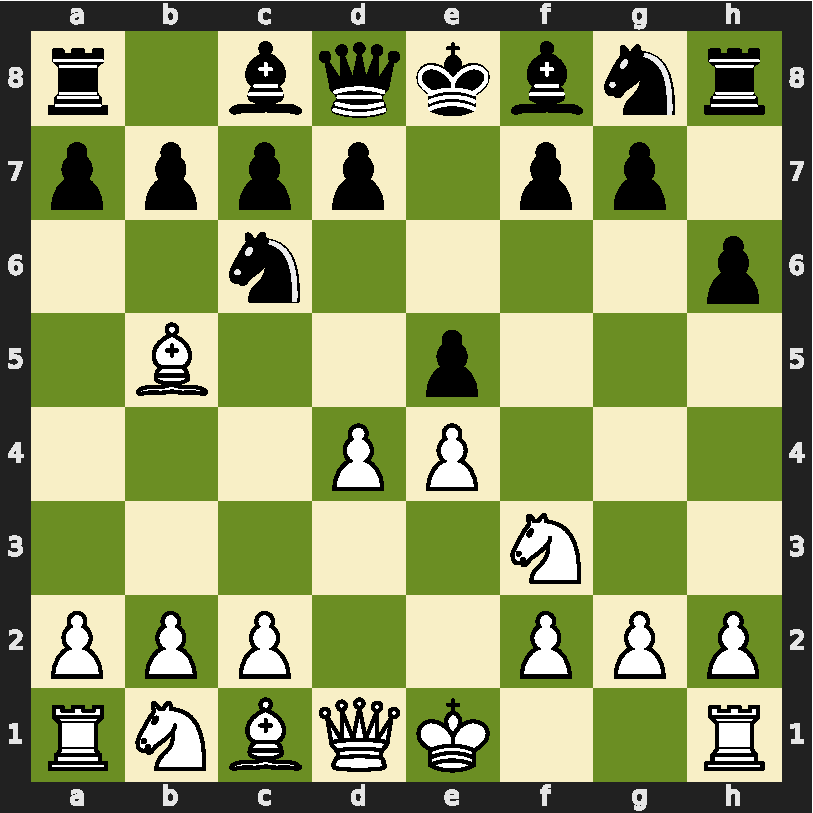
\includegraphics[width=\linewidth]{figures/board_next.pdf}
\end{subfigure}
\vspace{.1in}
\caption{Board state before (left) and after (right) the bishop at \pos{f1} is moved to \pos{b5}. UCI notation represents the move as \pos{f1b5}.}
\label{fig:move_notation}
\end{subfigure}
\vspace{-0.05in}
\caption{
Chess Notation %
}
\end{figure*}


Our results also provide some key insights on transformer language models:
\begin{enumerate*}[label=(\roman*)]
	\item They are robust to changes in input distribution where additional tokens, related to board state, are added to input sequence \emph{only during training} (Section~\ref{sec:rap_board}). 
	In contrast to LSTMs, transformers achieve this robustness even with smaller training sets (Section~\ref{sec:other_models}). 
	\item Even though chess is Markovian, the model relies on having access to the whole history, and the performance drops when limiting this access (Section~\ref{sec:limited_history}). 
\end{enumerate*}


\newpage
To summarize, our contributions are to: 

\begin{itemizesquish}
	\itemsep0em 
	\item Propose chess as a testbed for evaluating world state tracking capabilities of language models which can be used for development and analysis of these models.
	\item Show that with the appropriate chess notation, we can probe language models for aspects of the world state using simple prompts (Section~\ref{sec:probing}).
	\item Show that given enough training data, transformer language models can learn to track piece locations and predict legal moves with high accuracy.
	\item Demonstrate that transformer language models are robust to certain changes in input distribution, 
	and that access to world state during training improves performance with small datasets. 
 	
	 
	 
\end{itemizesquish}

